\documentclass{article}
\usepackage{enumitem}
\usepackage{graphicx}
\usepackage{microtype}
\usepackage{amsmath}
\usepackage[utf8]{inputenc}
\newcommand{\myskip}{\par\null\par}
\title{Math 305 Midterm 2}
\author{Theodore Koss}
\date{March 2023}
\begin{document}

\maketitle

\section*{Problem 1}
\begin{enumerate}[label=(\alph*)]
    \item Transition matrix: \newline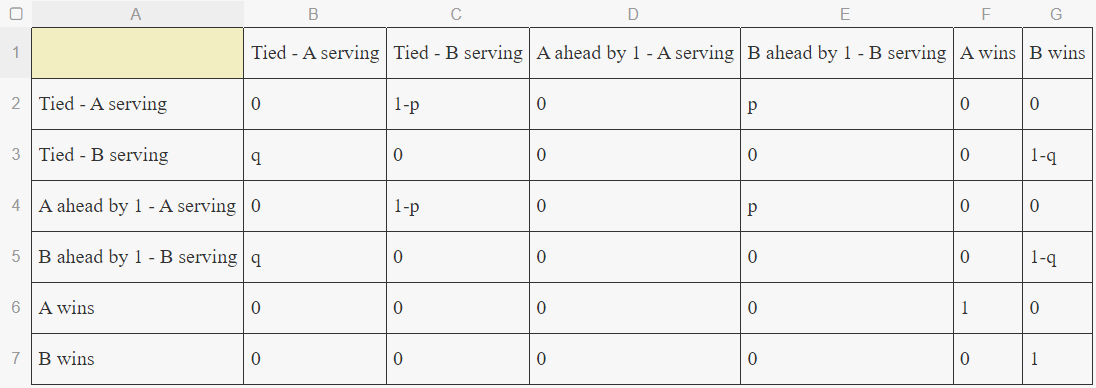
\includegraphics[scale=.35]{Pictures/Matrix1.png}
    \item Probability that the game will not be finished after four rallies is $0.0495+ 0.04095 = 0.09045$ or 9.04\%.
    \item Transition matrix:\newline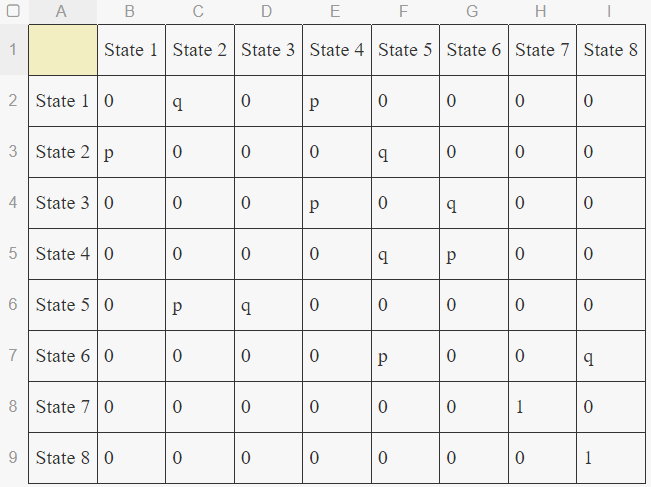
\includegraphics[scale=.375]{Pictures/Matrix2.png}
    \item Probability that game will not be finished after three rallies is $2.8\%$
\end{enumerate}
\section*{Problem 2}
\begin{itemize}
    \item Rank of page $A$: $.134$
    \item Rank of page $B$: $.118$
    \item Rank of page $C$: $.162$
    \item Rank of page $D$: $.059$
    \item Rank of page $E$: $.142$
    \item Rank of page $F$: $.147$
    \item Rank of page $G$: $.121$
    \item Rank of page $H$: $.118$
\end{itemize}
\section*{Problem 3}
\begin{enumerate}[label=(\alph*)]
    \item The paper discusses the formation of cell patterns in epithelial tissues and challenges the notion that the hexagonal cell pattern observed in simple epithelia is a result of optimal cell packing. The authors propose a mathematical model based on a discrete Markov chain to demonstrate that the distribution of polygonal cell types in epithelia is a consequence of cell proliferation rather than cell packing.
    \item $$f(t)=2f(t-1)$$ $$e(t)=e(t-1)+3f(t-1)$$ $$v(t)=v(t-1)+2f(t-1)$$ $$s(t) = \frac{(e(t-1) + 3 * f(t-1))}{f(t-1)}$$
    \item $\lim_{t\to \infty}{s(t)}=6$
    \item Transition matrix: \newline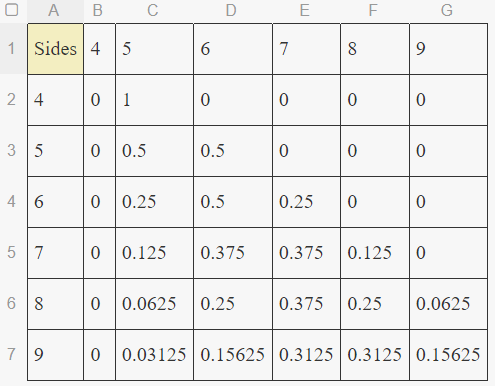
\includegraphics[scale=.35]{Pictures/Matrix3.png}
    \item Running this code gave the following results:\newline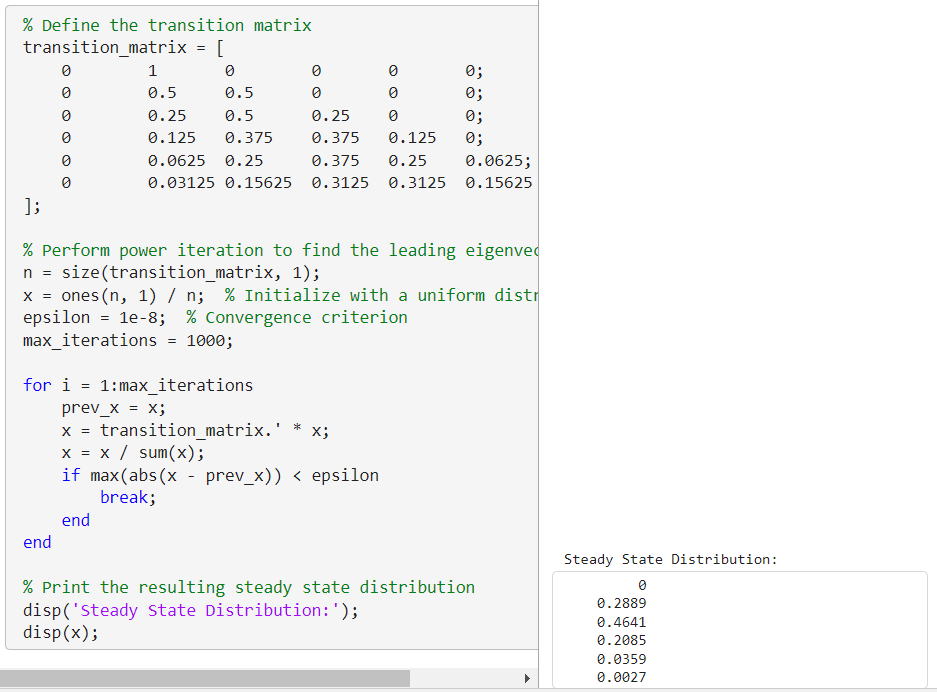
\includegraphics[scale=.5]{Pictures/Code.png}\begin{itemize}
        \item $28.89\%$ pentagons.
        \item $46.41\%$ hexagons.
        \item $20.85\%$ 7-gons.
        \item $3.59\%$ 8-gons.
        \item $0.27\%$ 9-gons.
    \end{itemize} This is almost exactly the results which the paper had.
\end{enumerate}
\end{document}